\documentclass[titlepage,11pt,twoside]{article}
\usepackage[dvips]{graphicx}

\usepackage[myheadings]{fullpage}
\usepackage{pmetrika}
%\usepackage{pmbib}

\usepackage{color}
\usepackage{mathtools}
\usepackage{amssymb}
\usepackage{hyperref}
\usepackage{natbib}
\usepackage{multirow}
%\usepackage{colortbl}
\usepackage[table]{xcolor}
\definecolor{lightgray}{gray}{0.9}
\usepackage[T1]{fontenc}

\usepackage{caption,setspace}
\captionsetup{font={footnotesize,stretch=1.5}}
\renewcommand{\baselinestretch}{2} 

\usepackage{tikz}
\usetikzlibrary{arrows}
\usetikzlibrary{shapes, positioning, calc} 


\newcommand{\bfU}{\mbox{\boldmath$\mathsf{U}$}}
\newcommand{\bfu}{\mbox{\boldmath$\mathsf{u}$}}
\newcommand{\hl}[1]{\textcolor{magenta}{#1}}
\newcommand{\RR}{\mathbb{R}}
\DeclareMathOperator*{\V}{V}
\DeclareMathOperator*{\argmax}{argmax}
\newcommand{\R}[1]{\texttt{#1}}
\newcommand{\acos}{\text{arccos}}


%\begin{figure}[h]
%\centerline{\includegraphics{figure03.eps}}
%\caption{Projection of item discrimination vectors onto $V_{\theta_T}$ hyperplance for a six item three-dimensional approximate sample structure.}
%\end{figure}

%\raggedbottom
\flushbottom


%\firstpage{1}
%\setcounter{lastpage}{999}
\setcounter{secnumdepth}{3}

\begin{document}

\begin{titlepage}
\linespacing{1}

\title{Exploratory data structure comparisons: Three new visual tools based on Principal Component Analysis}

\author{Anne H. Petersen}
\affil{Department of Public Health, University of Copenhagen}

\author{Bo Markussen}
\affil{Department of Mathematical Sciences, University of Copenhagen}

\author{Karl Bang Christensen}
\affil{Department of Public Health, University of Copenhagen}

\vspace{\fill}

\end{titlepage}\vspace*{24pt}



\Large{\textsc{Exploratory data structure comparisons: Three new visual tools based on Principal Component Analysis}}


\begin{center}\vskip3pt

\vspace{32pt}

Abstract\vskip3pt

\end{center}


\begin{abstract}
\linespacing{1}

In empirical psychometric work, one often encounters data that is somehow divided into two distinct subsets. This might be due to multi-center sampling frames, or to variations in instruments, orders of questionnaire item, modes of administration etc. Often, one wishes to combine such data into one and conduct only a single analysis, but this is only meaningful if the two subsets are similar in structures, that is, if they measure the same underlying concepts. However, procedures for assessing whether such a data collapsing is allowed are usually very ad hoc or require making full model assumptions. We present a suite of three visual, non-parametric diagnostic tools for investigating differences in data structures for two datasets containing different observations of the same variables, refered to as \textit{Principal Component Analysis-based Data Structure Comparisons} (PCADSC). This approach requires no directional nor hierarchical assumptions on the data. Since the tools are all based on Principal Component Analysis (PCA), they address differences in the structures of the covariance matrices of the two datasets, and by targeting different aspects of the PCA information, the three plots give a thorough and deep understanding of where differences occur and why it might be the case.

The functionality of the PCADSC tools is presented by use of data from the European Social Survey on psycological well-being in three European countries, namely Denmark, Sweden and Bulgaria. Here, we find that the concepts of psychological well-being are not the same when comparing Denmark and Bulgaria, and thus a comparison of e.g. mean scores in different well-being aspects is not meaningful. However, when comparing the two Scandinavian countries, Denmark and Sweden, we find very similar data structures and thus very similar concepts of well-being. Therefore, inter-country comparisons are warranted for these two countries. 

\begin{keywords}
multi-center studies, data heterogeneity, data structure comparisons, principal component analysis (PCA), European Social Survey.
\end{keywords}
\end{abstract}

\vspace{\fill}\newpage

\section{Introduction}
\label{sec:introduction}

Data comparability is a classical topic in statistics and a recurring one in psychometrics. Often, psychometric data will be collected in such a way that it is essentially divided into several subsets whose comparability (and thus collapsibility) needs to be assessed empirically. This happens e.g. when data are collected across several centers (or countries) or when different versions of an instrument, the mode of administration or the order of survey questionnaire items are applied. All of these practices are essential parts of the psychometric methodology, as it allows us to simultaneously build on existing methods and answer new, empirical questions. However, if we do not address the question of collapsibility among the data subsets arriving from e.g. different countries, we risk conducting analyses whose most fundamental assumptions are not satisfied. 

Sophisticated methods for addressing this question are available when we are willing to assume a statistical model. But this places the effort of assessing data comparability very late in the data analysis process and it makes the comparability assessment %very 
ad-hoc, as it essentially relies on the appropriateness of the modeling choices, which again depends on the structure of the data. The use of (parametric) models does thus not constitute a %valid 
general data structure comparison method, but rather a fitted-model comparison method. It addresses the interplay between the model and the data, not the data alone. However, useful tools for initial, exploratory investigations of data comparability that help researchers identify potential problems or challenges early in the study design development are mostly absent. What is needed is a procedure that compares differences in overall data structures in two (or more) subsets of a dataset without assuming neither directional nor hierarchical relationships between the variables. Simple methods like variable-by-variable tests in distributional differences suffer from the drawback that they only address marginal differences and ignore the interplay between variables. On the other hand, e.g. entry-by-entry comparisons of the two empirical correlation matrices quickly become unmanageable as the number of variables increase. 

While the issue is not in any way new, its relative importance is increasing due to new developments in data availability and data collection. Classical statistical methods are generally aimed at analyzing data from designed experiments and historically, statistical analyses have been conducted by researchers who knew the design and the source of the dataset well. However, the origin stories of datasets have changed over time and today, a lot of data are accumulated without a specific purpose in mind, as data collection and sharing has become easier and more affordable through the development of new technologies. This new era of data sharing facilitates a tremendous amount of new research, as data on all sorts of topics are now readily available online for %all
everyone to use. However, large scale publicly available datasets, such as the PISA data and European Social Survey (ESS) data, are often used by data analysts that are far removed from the data producers and therefore, problem-specific recommendations about e.g. potential instrument-induced challenges in the datasets %are not
may not be available for these data analysts. For this reason, a thorough investigation of data structure comparability becomes a crucial step in any meaningful data analysis when using such open-source data. 

The data structure comparison problem is however not limited to the context of new data sharing platforms. Even in single-population survey studies, a mixture of modes of administration is often used, e.g. mail and telephone, and while this can improve response rates, it can also be quite problematic \citep{Brambilla1987, McHorney1994}, and differences in response behavior can lead to biased results. Powers, Mishra and Young \citeyearpar{Powers2005} report effects of mode of administration on changes in mental health scores that are of a magnitude that is considered to be clinically meaningful, so the comparability issue is not just a statistical puzzle. Similarly, combining data obtained from different sampling schemes can also be problematic, as illustrated by Liu \citeyearpar{Liu2016}, who warns against the combination of online panel data (i.e. pre-recruited profiled pools of respondents) with intercept samples (a pool of respondents obtained through banners, ads, or promotions). 

The comparability issue that is present in all the examples presented so far can be summarized as follows: Assume that we have two datasets with the same variables, but different observations, or alternatively (and equivalently) a single dataset with a subset-inducing variable. Assume next that we wish to compare data structures without specifying a model, or even a variable of interest. The central question is then whether the two datasets can readily be combined for the purpose of later data analysis, or if the subset-inducing variable implies heterogeneity that must be somehow be dealt with, either in terms of modeling choices or simply by conducting several separate analyses.

We propose a suite of three new tools for this task, which we will refer to collectively as Principal Component Analysis-based Data Structure Comparisons (PCADSC). These methods employ the principal component decomposition of the empirical covariance matrix performed on two subsets of a dataset in order to create intuitive visualizations of data structure differences. 
%This yields a solution that is largely independent of the sizes of the two subsets of data. Anne: Det ved vi da ikke om det gør? Er det ikke netop det, vi siger, at man burde teste som næste step?
The proposed tools are implemented in the statistical software \texttt{R} in our package, \texttt{PCADSC} \citep{PCADSC}. 

This manuscript describes the procedures, including a brief introduction to principal component analysis (PCA), and presents a worked data example using open source, online available data on psychological well-being in three European countries from the European Social Survey. More specifically, we compare data from Denmark with data from Bulgaria and Sweden, respectively, to investigate whether or not data on psychological well-being can be combined across countries - a question that is completely ignored e.g. when international rankings of happiness among countries are posted by the UN \textit{World Happiness Report} project \citep{WHR2016}.




\section{PCA-based tools for data structure comparisons}
\label{sec:pcadscintro}
As mentioned above, the purpose of PCADSC is to compare overall data structures in two subsets of a dataset. But before we can get further into describing the PCADSC tools, we must first define the exact meaning of \textit{overall structures} in this context. One such definition is the structure of the covariance matrix of the dataset. If we assume all variables in the dataset to be jointly normal with known means, the covariance matrix is a sufficient statistic for describing the joint distribution of all the variables. 
%This gives it a very nice interpretation as a measure of the overall structure. If we do not accept 
And without the normality assumption, pairwise correlations and marginal variable variances are still interesting quantities that say something about the interrelations between the variables in the data. All in all, the empirical covariance matrix is a reasonable place to start looking for differences in \textit{overall data structures}.

A naive approach for data structure comparisons might therefore be to compute the empirical covariance matrices on each of the two data subsets and simply compare these matrices entry-by-entry. Though the idea perhaps sounds appealing at first, it is quite difficult to assess similarity of matrices, and moreover, it becomes increasingly difficult for large numbers of variables and thus high dimensional covariance matrices. There is simply too much information to consider at once. However, by use of linear algebra, we can decompose and recompose the covariance matrix such that the distinct dimensions of information withheld in it are clearly separated and ordered according to their relative importance. In particular, we find a new representation of the covariance matrix that makes it possible to gain an overview of the most interesting aspects of the data. One such decomposition strategy is known as \textit{principal component analysis} (PCA), which uses eigenvalue decomposition in order to obtain a new representation of the covariance matrix.

At this point a general remark about standardization is in place. PCA deconstructs the covariance matrix in components according to the most explained variance. This implies that if a variable has a very large sample variance (possibly because of its scale), this variable will always be deemed highly influential, no matter the structure of the data. Therefore, the variables are typically standardized prior to performing PCA. Note that the covariance matrix of the standardized variables is the same as the correlation matrix of the original variables, so post-standardization PCA simply corresponds to performing data structure comparisons of the correlation matrices rather than the covariance matrices. The standardization makes the variables comparable on the same scale, i.e.\ units of standard deviation. In this paper we will adopt this standardization policy, and in particular, we will allow for differences between scalings of the original, raw variables in the two data subsets.

%\hl{Bo: I næste afsnit bruges stadigvæk ``covariance''. Det er vel ok?} Anne: Synes det fungerer fint.

\subsection{A brief introduction to principal component analysis}
Consider $n$ observations $x_1,\dotsc,x_n \in \RR^d$ of $d$ variables, let $\bar{x} = (\bar{x}_1, ..., \bar{x}_d)^\top = \frac{1}{n} \sum_{i=1}^n x_n$ denote their averages, and let $S = \frac{1}{n-1} \sum_{i=1}^n (x_i-\bar{x}) (x_i-\bar{x})^\top \in \RR^{d \times d}$ denote the empirical covariance matrix of the full data matrix, $X$. We assume in the following that all variables of $X$ have a numerical interpretation, e.g. by being continuous or ordinal and categorical. For a given $q \leq d$, principal component analysis (PCA) is a tool for finding a new representation of the dataset of dimension $q$ such that the least possible amount of information is lost. More specifically, we wish to minimize the loss when looking at a projection of $X$ onto a $q$-dimensional space, rather than the original $d$-dimensional one. Formally, we define the \emph{rank-q-reconstruction error} as the minimal squared error that is achievable by linear subspaces $K_q \subset \RR^d$ of dimension $q < d$, that is
\begin{equation*}
\min_{K_q} \sum_{i=1}^n \min_{z \in K_q} \lVert x_i - \bar{x} - z \rVert^2 =
\min_{K_q} \sum_{i=1}^n \lVert x_i - \bar{x} - \text{proj}_{K_q}(x_i - \bar{x}) \rVert^2.
\end{equation*}
The theory of \emph{Principal component analysis} (PCA) not only ensures the existence of a subspace $\hat{K}_q \subset \RR^d$ that attains this minimum, it also provides an explicit description of $\hat{K}_q$ and the rank-q-reconstruction error \citep{HastieEtAl2009}. More specifically, the rank-q-reconstruction error is attained when we choose
\begin{equation*}
\hat{K}_q = \text{span}\{\eta_1,\dotsc,\eta_q\},
\end{equation*}
where $\eta_1, ..., \eta_q$ are the $q$ first eigenvectors of the empirical covariance matrix, $S$, as ordered by the size of their associated eigenvalues, $\lambda_1, \dotsc, \lambda_d$. In the PCA framework, we refer to the eigenvectors as \textit{loadings}. The eigenvalues may be understood as \textit{variance components}, as the sum of the marginal empirical variances is preserved under eigenvalue decomposition, that is,
\begin{equation*}
\text{trace}(S) = \sum_{j=1}^d \hat{V}(x_j) = \sum_{j=1}^d \hat{V}(\eta_j^\top X^\top) = \sum_{j=1}^d \lambda_j,
\end{equation*}
where $x_j \in \RR^n$ 
%\hl{(Bo: $X_1$ og $X_2$ bruges i en anden betydning i afsnit 2.2. Omformuler?)} Anne: Hov, ja, hermed x_j så det passer med notationen ovenfor.
denotes the $j$th variable of $X$ and $\hat{V}$ is the empirical variance function. This again emphasizes that we do not change the covariance structure of a dataset when performing PCA; we merely use linear algebra to make it easier to describe. And as eigenvalues are uniquely defined, and eigenvectors are uniquely defined up to a change of sign whenever the eigenvalues are %different,
distinct, the representation hereby obtained is a valid object of inference. If $n < d$ or if the covariance matrix does not have full rank, it is possible to obtain non-unique eigenvalues, e.g.\ $\lambda_i=\lambda_{i+1}=\dotsm=\lambda_j$, but even in this case, the associated eigenvectors $\eta_i,\eta_{i+1},\dotsc,\eta_j$ are uniquely defined up to a common rotation.

The $j$th loading can also be found iteratively as the unit vector $u \in \RR^d$ orthogonal to $\hat{K}_{j-1}$ that maximizes the variation of the associated scores:
\begin{align*}
\eta_j &= \argmax_{u \in \RR^d\colon u \perp \hat{K}_{j-1}} \sum_{i=1}^n \lVert u^\top (x_i - \bar{x}) \rVert^2, &
\lambda_j &= \frac{1}{n-1} \sum_{i=1}^n \lVert \eta_j^\top (x_i - \bar{x}) \rVert^2,
\end{align*}
where the initial subspace is defined as $\hat{K}_0 = \{0\}$. It is worth emphasizing that this greedy approach of successively adding the next direction $\eta_j$ explaining most of the remaining variation also gives the sequence $\hat{K}_q = \hat{K}_{q-1} \oplus \text{span} \{\eta_q\}$ of subspaces minimizing the rank-q-reconstruction error. This strong interpretation of PCA, which is often overlooked in the literature, means that the sequence of loadings $\eta_j$ and their associated variation components $\lambda_j$ yield a simultaneous description of the structure of the dataset for all approximating dimensions $q$. This implies that the loadings and the variation components can be used to investigate the structure of the dataset without the need to decide on an approximating dimension, $q$, a priori.

\subsection{Using PCA for data structure comparisons}
\begin{figure}
\center 
Model 1: \medskip \\
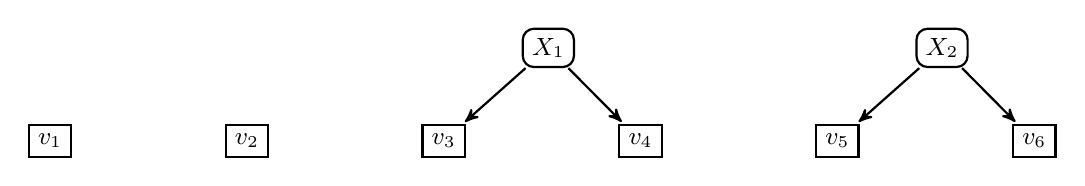
\begin{tikzpicture}[->,>=stealth',shorten >=1pt,auto, node distance=2.5cm,
  thick,main node/.style={rectangle, rounded corners,draw,font=\sffamily\small\normalfont},
  sq node/.style={rectangle,draw,font=\sffamily\small\normalfont}]
  \node[sq node] (1) {$v_1$};
  \node[sq node, right of = 1] (2) {$v_2$};
  \node[sq node, right of = 2] (3) {$v_3$};
  \node[sq node, right of = 3] (4) {$v_4$};
  \node[sq node, right of = 4] (5) {$v_5$};
  \node[sq node, right of = 5] (6) {$v_6$};
  \node[main node, above right=1cm of 3] (7) {$X_1$};
  \node[main node, above right=1cm of 5] (8) {$X_2$};
  \path[every node/.style={font=\sffamily\small}]
    (7) edge node  {} (3)
    (7) edge node {} (4)
    (8) edge node {} (5)
    (8) edge node {} (6);
 \end{tikzpicture}
\\
\bigskip
Model 2: \medskip \\
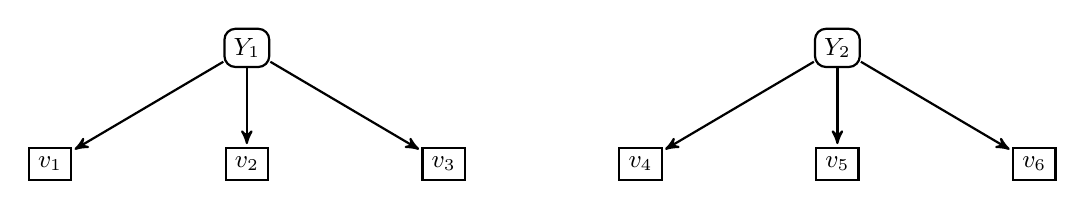
\begin{tikzpicture}[->,>=stealth',shorten >=1pt,auto, node distance=2.5cm,
  thick,main node/.style={rectangle, rounded corners,draw,font=\sffamily\small\normalfont},
  sq node/.style={rectangle,draw,font=\sffamily\small\normalfont}]
  \node[sq node] (1) {$v_1$};
  \node[sq node, right of = 1] (2) {$v_2$};
  \node[sq node, right of = 2] (3) {$v_3$};
  \node[sq node, right of = 3] (4) {$v_4$};
  \node[sq node, right of = 4] (5) {$v_5$};
  \node[sq node, right of = 5] (6) {$v_6$};
  \node[main node, above=1cm of 2] (7) {$Y_1$};
  \node[main node, above=1cm of 5] (8) {$Y_2$};
  \path[every node/.style={font=\sffamily\small}]
    (7) edge node  {} (1)
    (7) edge node {} (2)
    (7) edge node {} (3)
    (8) edge node {} (4)
    (8) edge node {} (5)
    (8) edge node {} (6);
 \end{tikzpicture}
\caption{Graphical representations of the two models that are used for simulating example data for the PCADSC plots. Square nodes represent observed variables, while rounded nodes represent latent variables.  Arrows are used to illustrate causal links, and thus we e.g. find in \textit{Model 1} that the observed variables $v_3$ and $v_4$ are caused by a common, unobserved variable, namely $X_1$. Further details on the models and the simulated data are available in Appendix \ref{appendix.simData}, including covariance matrices for the two models.}
\label{fig.simGraphs}
\end{figure}


All in all, PCA qualifies as an appealing first step in structural comparisons of two datasets containing the same variables, and especially the loadings and variance components are meaningful and interesting objects to compare across such different datasets. Usually, when performing PCA with other purposes in mind, the main interest lies in the \textit{scores}, i.e. the projections $\eta_j^\top (x_i - \bar{x})$ of the observations onto the loadings. But where the scores describe the observations, the variation components and the accompanying loadings describe the usage of the variables. If two different datasets with the same variables, but different samples of observations, have similar loading patterns, then the variables appear to be measuring the same underlying quantities in both datasets. This can be the case while the two sets of scores could be arbitrarily different, which could e.g.\ happen if the two datasets were taken from two different populations of subjects. On the other hand, if the loading patterns are different in the two datasets, then this indicates that the variable interplay differs in the two data situations, and hence it would be criticizable to use these variables for comparisons across the two datasets.

The tools presented in this paper are all based on comparing the PCA results across two different datasets that contain the same variables. We denote these two datasets by $X_1$ and $X_2$, respectively, with $X_1$ consisting of $n_1$ observations of $d$ variables $x_{11},\dotsc,x_{1 n_1} \in \RR^d$, and similarly, $X_2$ consisting of $n_2$ observations of the apparently same $d$ variables, $x_{21},\dotsc,x_{2 n_2} \in \RR^d$. %
Furthermore, let $X$ be the combined dataset consisting of all $n=n_1+n_2$ observations. For these %two
three datasets, we complete the following steps:
\begin{enumerate}
\item Within each dataset, standardize each of the variables to have mean zero and unit standard deviation. Let $\tilde{x}_{ij} \in \RR^d$ for $i=1,2$ and $j=1,\dotsc,n_i$ and $\tilde{x}_j \in \RR^d$ for $j=1,\dotsc,n$ be the standardized datasets.
\item Form the principal component analyses
\begin{align*}
S_i &= \frac{1}{n_i-1} \sum_{j=1}^{n_i} \tilde{x}_{ij} \tilde{x}_{ij}^\top = \sum_{k=1}^d \lambda_{ik} \eta_{ik} \eta_{ik}^\top \quad \text{for $i=1,2$,} &
S &= \frac{1}{n-1} \sum_{j=1}^n \tilde{x}_j \tilde{x}_j^\top = \sum_{k=1}^d \lambda_k \eta_k \eta_k^\top,
\end{align*}
thereby obtaining loadings $\eta_{1k}, \eta_{2k}, \eta_k$ and variance components $\lambda_{1k}, \lambda_{2k}, \lambda_k$ for $k=1,\dotsc,d$.
\end{enumerate}
The hereby obtained PCA decompositions of the correlation matrices can then be compared. We present three diagnostic plots that are designed to shine a light on different types and levels of data structure differences. These three plots are:
\begin{description}
\item[The CE plot:] The CE (cumulative eigenvalue) plot can be used to illustrate differences in variance components, that is, in the relative importance of the directions identified by the PCA. The CE plot is accompanied by two permutation-tests, testing the hypothesis of no difference in variance components.
\item[The angle plot:] The angle plot compares both loadings and variance components at once and it can be used to understand the information loss if the data structure of one dataset is superimposed on the other, thereby revealing which principal components (i.e. loading and variance component pairs) that are most similar and most different across the two datasets
\item[The chroma plot:] The chroma plot is primarily an illustration of the loading patterns and it targets the question of how the roles of the original variables are different between the two datasets, thus leading the data structure comparison question back to its original, empirical context.
\end{description}
For the deepest understanding of the data structure differences in two datasets, we suggest using all three steps in the above order.

Note that the standardization implies that the diagonal elements of $S$, $S_1$, and $S_2$ all equals 1, and thus also that
\begin{equation*}
\sum_{k=1}^d \lambda_k = \sum_{k=1}^d \lambda_{1k} = \sum_{k=1}^d \lambda_{2k} =  d.
\end{equation*}
This identity will simplify some expressions below.

While we present the three plot types from a purely theoretical point of view below, we also provide example illustrations as a supplement to the somewhat technical definitions. These plots are available in Figures \ref{plot.simCE}, \ref{plot.simAngle} and \ref{plot.simChroma} for the CE-, angle- and chroma plots, respectively, and they are based on two simulated datasets:
\begin{description}
\item[Dataset A:] This dataset contains 1000 independent simulations from the same underlying model, namely \textit{model 1} from Figure \ref{fig.simGraphs}. The observations are randomly divided into two groups.  
\item[Dataset B:] This dataset contains 500 independent simulations from \textit{model 1} from Figure \ref{fig.simGraphs} and 500 independent simulations from \textit{model 2} in the same figure. The observations are naturally divided into groups corresponding to which model they were simulated from.
\end{description} 
Further details about the data simulations are available in Appendix \ref{appendix.simData}. In dataset A, all observations stem from the same, underlying data structure and thus, the PCADSC plots should point towards no notable differences in data structures. In dataset B, on the other hand, there are two fundamentally different, underlying datastructures and therefore, the PCADSC plots should illustrate this lack of homogeneity in data structures.


\subsubsection{The cumulative eigenvalue plot}
\begin{figure}
\centerline{\includegraphics[scale = 0.65]{simCE2.pdf}}
\centerline{\includegraphics[scale = 0.65]{simCE1.pdf}}
\caption{CE plots for the two simulated datasets. Dataset A, which includes no differences in data structures, is found in the top panel, and dataset B, where the observations stem from two different underlying models, is presented in the bottom panel. Both plots are annotated with the $p$-values of the Kolmogorov-Smirnov and the Cram\'er-von Mises tests of the hypothesis of no difference in data structures. The bold, black lines illustrate the observed cumulative eigenvalue differences, while the shaded areas are 95 \% confidence bands under the null hypothesis of no difference in data structures. In the top panel, we see a cumulative eigenvalue curve that falls well within the confidence region, thereby suggesting no difference in eigenvalues (as expected). This also agrees with the large $p$-values and the fact that only a single underlying model was used for generating this data. In the bottom panel, the conclusion is reversed, which is also in accordance with the nature of the simulated data, which contains two distinct groups.}
\label{plot.simCE}
\end{figure}

The cumulative eigenvalue (CE) plot compares the variation components, i.e. the eigenvalues of the correlation matrix. These eigenvalues represent how much information is withheld in each component in terms of explained variance. Thus, by comparing cumulative sums of variance components, it is possible to obtain a detailed picture of how the two datasets differ in terms of what components are the most informative. 
%If these are the same in the two sample populations, then the best estimate for the variation components are $\lambda_1 \ge \dotsm \ge \lambda_d \ge 0$ found in the combined dataset. And we would expect $\lambda_{i1} \ge \dotsm \ge \lambda_{id} \ge 0$ for $i=1,2$ to be alike excepts sample variation.
In order to investigate whether the same proportion of the total variation can be described by the same number of principal components in the two datasets, we plot a piecewise linear curve connecting the points
\begin{align*}
(0,0), &&
(\lambda_1,\lambda_{11}-\lambda_{21}), &&
(\lambda_1 + \lambda_2,\lambda_{11}+\lambda_{12}-\lambda_{21}-\lambda_{22}), &&
\ldots, &&
\bigg( \sum_{j=1}^d \lambda_j, \sum_{j=1}^d \lambda_{1j} - \sum_{j=1}^d \lambda_{2j} \bigg)
\end{align*}
%This may be seen as a cumulative Bland-Altman plot \citep{AltmanBland83,LinEtAl2002} for the variation components.
%Anne: NK pointed out that this is somewhat confusing for people who are not familiar with the Bland-Altman plot, and as far as I can tell, what we do is quite different anyway, so I think no reference is really needed(?) 
Note that due to the standardization, the last point will always be equal to $(d,0)$. Thus, this curve will begin and end at the x-axis. And the larger excursions it makes away from the x-axis, the less alike the cumulative variation components for the two datasets are. Moreover, a positive cumulative difference implies that dataset 1 holds more information in the first components than dataset 2 does. Two examples of cumulative eigenvalue plots are available in Figure \ref{plot.simCE}.

In order to test whether these cumulative differences are statistical artefacts or if they represent something real, we have implemented both the \emph{Kolmogorov-Smirnov} and the \emph{Cram\'er-von Mises} test statistics, which are given by
\begin{align*}
\text{KS} &= \max_{k=1,\dotsc,d} \bigg\lvert \sum_{j=1}^k \lambda_{1j} - \sum_{j=1}^k \lambda_{2j} \bigg\rvert, &
\text{CvM} &= \sum_{k=1}^{d-1} \frac{\lambda_k + \lambda_{k+1}}{2} \bigg( \sum_{j=1}^k \lambda_{1j} - \sum_{j=1}^k \lambda_{2j} \bigg)^2.
\end{align*}
We conduct the tests as \textit{permutation tests}, that is, by randomly reallocating the combined and separately standardized datasets into two new datasets of $n_1$ and $n_2$ observations, respectively, and then redoing the CE plot steps and recalculating the test statistics. This should be done a large (e.g. 10000) number of times. Then, a $p$-value is obtained by computing the proportion of reallocated datasets that lead to %even larger 
test statistics at least as large as %than 
the one we found for the original datasets.

The permutation test results are also used to visualize the uncertainty of the CE curve in the plots. In the CE plots shown in the following section, we plot the observed curve together with 20 of the resampled curves, as well as a shaded region visualizing pointwise 95 \% coverage intervals. If the observed curve is very different from the resampled curves or if it is substantially outside the shaded region, then this also indicates differences between the two datasets.

%Whether the excursions in the observed curve are large or within the range of sample variation can be quantified by a permutation test. The idea is that we randomly reallocate the $n_1+n_2$ observations in the combined dataset to two datasets with $n_1$ and $n_2$ observations, respectively, and then repeat the procedure described above. The random reallocation by construction ensures that the two resampled datasets are alike except their sample size and sampling variation. In the \emph{CumEigenPlot} we make 1000 independent random reallocations, and plot  P-values for the null hypothesis that the variation components are the same are easily provided for any appropriate test statistic by the resampling procedure as well.

\subsubsection{The angle plot}
\begin{figure}
\centerline{\includegraphics[scale = 0.65]{simAngle2.pdf}}
\centerline{\includegraphics[scale = 0.65]{simAngle1.pdf}}
\caption{Angle plots for the two simulated datasets, with dataset A in the top panel and dataset B in the bottom panel. The blue show the principal components of the observations in group 1 decomposed in the coordinate system of the principal components of group 2, while the red arrows illustrate the reverse. For dataset A, we find very short off-diagonal arrows, suggesting that the two PCA decompositions agree on the relative placement of the information in  the data among the 6 PCs.  For dataset B, on the other hand, we find very little agreement in all components, which should be expected, as the two groups in the dataset correspond to different data structures.}
\label{plot.simAngle}
\end{figure}

This plot simultaneously compares the variation components and the loadings. Let $\lambda_{\max} = \max\{ \lambda_{11}, \lambda_{21} \}$ be the largest variation component for the two datasets. Then the empirical correlation matrix for the first dataset, $S_1$, has the following orthogonal decomposition in the coordinate system of the second dataset
%\begin{equation*}
%S_1 = \sum_{k=1}^d \lambda_{1k} \eta_{1k} \eta_{1k}^\top
%= \lambda_{\max} \sum_{k=1}^d
%\Bigg( \sum_{j=1}^d \sqrt{\frac{\lambda_{1k}}{\lambda_{\max}}} (\eta_{1k} \eta_{2j}^\top) \eta_{2j} \Bigg)
%\Bigg( \sum_{j=1}^d \sqrt{\frac{\lambda_{1k}}{\lambda_{\max}}} (\eta_{1k} \eta_{2j}^\top) \eta_{2j} \Bigg)^\top,
%\end{equation*}
\begin{equation*}
S_1 = \sum_{k=1}^d \lambda_{1k} \eta_{1k} \eta_{1k}^\top
= \lambda_{\max} \sum_{k=1}^d
\Bigg( \sum_{j=1}^d \sqrt{\frac{\lambda_{1k}}{\lambda_{\max}}} \eta_{2j} (\eta_{2j}^\top \eta_{1k}) \Bigg)
\Bigg( \sum_{j=1}^d \sqrt{\frac{\lambda_{1k}}{\lambda_{\max}}} \eta_{2j} (\eta_{2j}^\top \eta_{1k}) \Bigg)^\top,
\end{equation*}
and we have a similar decomposition of $S_2$ in the coordinate system of the first dataset %\hl{Anne: it was not completely clear to me what this meant the first xx times I read it - expand? Bo: Jeg har ikke noget bud på en sådan udvidelse lige nu og her --- skal vi ikke bare sige at det er ok i sin nuværende form?}.
We propose to visualize these two decompositions in a $d \times d$ grid display. In the $j$th row and $k$th column of this display we plot two arrows based at the lower left corner of the grid cell. The first arrow has length $\mu_{jk}$ and angle $\theta_{jk}/2$ counterclockwise from the diagonal, and the second arrow has length $\nu_{jk}$ and angle $\theta_{jk}/2$ clockwise from the diagonal. To facilitate the following description we will refer to the arrows drawn counterclockwise as the blue arrows, and the arrows drawn clockwise as the red arrows. The lengths $\mu_{jk}$ and $\nu_{jk}$ and the angle $\theta_{kj}$ are given by
\begin{align*}
\mu_{jk} &= \sqrt{\frac{\lambda_{1k}}{\lambda_{\max}}} \lvert \eta_{1k}^\top \eta_{2j} \rvert, &
\nu_{jk} &= \sqrt{\frac{\lambda_{2j}}{\lambda_{\max}}} \lvert \eta_{2j}^\top \eta_{1k} \rvert, &
\theta_{jk} &= \acos(\lvert \eta_{1k}^\top \eta_{2j} \rvert).
\end{align*}
Note that for two $d$-dimensional, unit length vectors $a$ and $b$, it holds that $ a^\top b = \langle a, b \rangle = \tilde{c}(a,b)$, where $\tilde{c}$ denotes the sample correlation. Thus, in the angle plot, we are essentially looking at the absolute values of correlations between loadings that have been scaled according to their variance component contributions. The absolute value of the projection $\eta_{1k} \eta_{2j}^\top$ is inserted due to the indeterminacy of the direction of loading vectors. This indeterminacy implies that the angle between loadings from the two datasets always can be chosen to be in the interval $[0,\pi/2]$, and hence the decomposition of $S_1$ and $S_2$ can be visualized in a joint plot by dividing the angles by two and using counterclockwise and clockwise shifts from the diagonal. Furthermore, the scaling of the lengths by $\lambda_{\max}$ is made so that the longest arrow has at most unit length. Figure \ref{plot.simAngle} presents two examples of angle plots based on simulated data.

In the \emph{angle plot}, the blue arrows in the $k$th column of the grid display visualize the decomposition of the $k$th principal component of the first dataset in the coordinate system of the second dataset. Similarly, the red arrows in the $j$th row visualize the decomposition of the $j$th principal components of the second dataset in the coordinate system of the first dataset. %\hl{Can we expand on this in a non-technical way? - Karl: it seems that we cannot}
If the structures of the two datasets are identical, then we will have coinciding blue and red arrows along the diagonal in the grid display, and nothing else as arrows in the off-diagonal cells would have zero length. Differences in the variation components are visualized as differences in the lengths of the blue and the red arrows, also in the diagonal. And loadings in other directions than the corresponding loading from the other dataset are visualized as angle separation of the blue and the red arrows in the diagonal cells, as well as arrows of non vanishing length in the off-diagonal cells.


\subsubsection{The chroma plot}
\begin{figure}
\centerline{\includegraphics[scale = 0.65]{simChroma2.pdf}}
\centerline{\includegraphics[scale = 0.65]{simChroma1.pdf}}
\caption{Chroma plots for the two simulated datasets, with dataset A in the top and dataset B in the bottom. Each bar represents a principal component and the bars are annotated with their cumulative percentages of explained variance ($\tilde\sigma_{ij}^c$). For dataset A, we see very similar visual patterns across the two panels, corresponding well with the fact that both groups are drawn from the same underlying model. For dataset B, we see different color compositions for the bars in the left- and the right panel, illustrating that the data structures are not identical for the two groups.}
\label{plot.simChroma}
\end{figure}

This plot compares the loadings of the two datasets. The chroma plot consists of two panels, one for each dataset, made up of colored bars. These bars each represent a principal component and their coloring illustrates the relative weights of the $d$ original variables, that is, their absolute, normalized loading contributions. More specifically, when illustrating the $i$th principal component in the two data subsets, we plot vertical bars of length one that has been divided into $d$ segments of different colors. The width of the $j$th colored segments are given by
\begin{align*}
\omega_{1ij} &= \frac{\lvert\eta_{1ij}\rvert}{\sum_{k=1}^d \lvert\eta_{1ik}\rvert}, &
\omega_{2ij} &= \frac{\lvert\eta_{2ij}\rvert}{\sum_{k=1}^d \lvert\eta_{2ik}\rvert},
\end{align*}
where $\eta_{1ij}$ and $\eta_{2ij}$ denotes the $j$th entry of $\eta_{1i}$ and $\eta_{2i}$, respectively. Due to the indeterminacy of the sign, all the signs are removed from the coefficients in the loadings. The bars are ordered according to the variation components and they are annotated with the cumulative percentage explained variance of that component, that is, the scaled and summed variance component contributions,
\begin{align*}
\tilde\sigma^c_{1i} &= \frac{\sum_{j=1}^i \lambda_{1j}}{\sum_{k=1}^d \lambda_{1k}} = \frac{\sum_{j=1}^i \lambda_{1j}}{d}, &
\tilde\sigma^c_{2i} &= \frac{\sum_{j=1}^i \lambda_{2j}}{\sum_{k=1}^d \lambda_{2k}} = \frac{\sum_{j=1}^i \lambda_{2j}}{d}.
\end{align*}
Especially when $d$ is large, we recommend plotting only a select set of interesting principal components, e.g. as identified by use of the angle plot. In this scenario, the annotations should rather be the non-cumulative variance contributions, $\tilde\sigma_{1i} = \frac{\lambda_{1i}}{d}$ and $\tilde\sigma_{2i} = \frac{\lambda_{2i}}{d}$. In Figure \ref{plot.simChroma}, two examples of chroma plots are available. 

The plots resulting from this procedure should be inspected focusing on two properties: Similarities in loading patterns, which will correspond to similar visual impressions, and similarities in variance contributions. For each component, the loadings describe how influential the different variables are on that component. Therefore, the chroma plot allows us to make qualitative statements about the original datasets, such as \textit{"variable $x$ is generally more influential in subset 1 than it is in subset 2"}, thereby helping us to understand where and why potential data structure differences are found.


\section{Comparing psychological well-being: A data example}
\label{sec:dataexample}
We will now turn to a concrete data example in order to illustrate the capabilities of the tools presented above. We use data from the 2012 version of the European Social Survey (ESS) project to investigate inter-country differences in psychological well-being and happiness. The topic of our investigation is motivated by an increasingly popular tendency to publish rankings of countries in fields as different as educational quality (e.g. the PISA project) and citizen happiness (e.g. the UN \textit{World Happiness Report} project). From a methodological point of view, such international rankings are very problematic, as they rely on the fundamental assumption that the measured concepts are inherently the same across countries. The PCADSC tools qualify as a suite of methods for exploring the validity of this assumption empirically. 

In the rankings of happiness, not much work has yet been devoted to evaluating the assumption of international comparabiltity, though \cite{Veenhoven2012} presents a theoretically thorough, but empirically simplistic, summary of possible reasons for lack of comparability, while \cite{Lolle2016} show highly potent translation issues for the term \textit{happiness}. But the problem is beyond translation efforts: The main question really is whether or not there exist such a thing as a universal, internationally valid concept of happiness. If not, the very idea of translation is meaningless, since different aspects of psychological well-being or happiness simply do not have the same relative meaning in different cultural and socio-economic settings. This is in fact a question concerning comparability of data structures. If two countries differ e.g. in terms of how social networks are typically built and structured, with one emphasizing family relations and the other mostly focusing on other social relations, then having a weak family connection does not have the same implications in the first country as it does in the second one. More specifically, whereas in the first country, lack of familial network might be related to loneliness, lack of general social capital and isolation, in the second country, the quality of the family network might not be informative at all about other aspects of a person's social or psychological well-being. The two countries thus differ in how different aspects or measures of psychological well-being are interrelated, which is essentially a difference in data structures. And therefore, comparing the two countries in these measures is not a meaningful endeavor. 

In this section, we use the PCADSC tools to examine international differences in one aspect of happiness, namely psychological well-being. Our starting point is Denmark, a small, Northern European country that has repeatedly been awarded with the title of ``happiest country in the world''  by the \textit{World Happiness Report}, most recently in 2016 \citep{WHR2016}, and we wish to investigate if this title is really meaningful at all. In order to do this, we compare the Danish ESS psychological well-being data with that of Bulgaria. Though both countries are European and thus neither very far apart geographically nor culturally, these two countries have previously been highlighted to be very different in terms of what defines happiness \citep{ESStopline5}. Moreover, intra-European, regional differences in the relationship between social capital and happiness have also been demonstrated \citep{Rodriguez2014}. When comparing Northern European countries to other European countries, a much less pronounced relationship between the two concepts is found. In particular, interpersonal relations play a less important role in Denmark, compared to Bulgaria. Therefore, a successful method for data comparisons should be able to detect these differences by looking at data on psychological well-being from these two countries.

We also compare the Danish data with Swedish data in order to investigate if the PCADSC tools actually do hold discriminatory power. Denmark and Sweden are both Northern European countries and are often deemed very similar in terms of culture and history. Therefore, we expect fundamental concepts, such as psychological well-being, to be similar across these two countries.

All computations and figures presented in this section were created using our \R{R} package \R{PCADSC} \citep{PCADSC}. 

\subsection{Data}

\begin{table}[t]
\centering
%\begin{tabular}{lccccccccc}
%  \hline
%  & \multicolumn{3}{c}{Denmark} & \multicolumn{3}{c}{Bulgaria} & \multicolumn{3}{c}{Sweden} \\
% & $Q_1$ & $M$ & $Q_3$ \quad & $Q_1$ & $M$ & $Q_3$ \quad & $Q_1$ & $M$ & $Q_3$ \\
%  \hline
% Evaluative wellbeing & 8.00 & 8.75 & 9.50 & 3.50 & 5.00 & 7.00 & 7.00 & 8.00 & 9.00 \\
% Emotional wellbeing & 7.22 & 8.33 & 8.89 & 5.00 & 6.67 & 7.78 & 6.67 & 7.78 & 8.89 \\
%Functioning & 6.93 & 7.57 & 8.21 & 5.50 & 6.68 & 7.68 & 6.39 & 7.04 & 7.68 \\
%Vitality & 6.67 & 7.50 & 8.33 & 5.83 & 7.50 & 8.33 & 6.67 & 7.50 & 9.17 \\
% Community wellbeing & 5.83 & 6.77 & 7.57 & 3.70 & 4.67 & 5.70 & 5.66 & 6.57 & 7.37 \\
%Supportive relationships & 7.42 & 8.25 & 8.92 & 6.17 & 7.25 & 8.08 & 7.42 & 8.25 & 8.75 \\
%   \hline
%\end{tabular}
\begin{tabular}{lccc}
  \hline
  & Denmark & Bulgaria & Sweden \\
  \hline
 Evaluative wellbeing & 8.75 (8.00, 9.50) & 5.00 (3.50, 7.00) & 8.00 (7.00, 9.00) \\
 Emotional wellbeing & 8.33 (7.22, 8.89) & 6.67 (5.00, 7.78) & 7.78 (6.67, 8.89) \\
Functioning & 7.57 (6.93, 8.21) & 6.68 (5.50, 7.68) & 7.04 (6.39, 7.68) \\
Vitality & 7.50 (6.67, 8.33) & 7.50 (5.83, 8.33) & 7.50 (6.67, 9.17) \\
 Community wellbeing & 6.77 (5.83 ,7.57) & 4.67 (3.70, 5.70) & 6.57 (5.66, 7.37) \\
Supportive relationships & 8.25 (7.42, 8.92) & 7.25 (6.17, 8.08) & 8.25 (7.42, 8.75) \\
   \hline
\end{tabular}

\caption{Median values of each of the six dimensions of psychological well-being, stratified by country. 25 and 75 percentiles are listed in parentheses. Note that the scales are constructed such that they all run from 0-10.}
\label{tableDistr}
\end{table}

The ESS 2012 data contain a total of 626 variables collected from 54673 citizens of 29 countries. Here, we will only work with a subset of 35 questionnaire items that are all related to psychological well-being. These 35 items can be divided into 6 distinct scales, namely \textit{Evaluative wellbeing}, \textit{Emotional wellbeing}, \textit{Functioning}, \textit{Vitality}, \textit{Community wellbeing} and \textit{Supportive relationships}. More details on these scales can be found in \citep{ESStopline5} and the relationship between questionnaire items and scales is summarized in Table \ref{table:items} in the appendices. We represent each of the scales by a single variable, which is calculated as the average score within the items related to that variable and scaled such that it takes a value between 0 and 10. For simplicity, we use only complete cases for this construction and thus exclude all participants that did not answer all the 35 questionnaire items used below. This corresponds to approximately 9\% of the observations in the Danish sample, 20\% in the Bulgarian sample and only 6\% in the Swedish sample. All in all, we have $n_{DK} = 1498$ complete case observations in the Danish sample, $n_{BG} = 1798$ observations in the Bulgarian sample and $n_{SE} = 1736$ Swedish observations. Table \ref{tableDistr} summarizes the marginal distributions of the six dimensions of psychological well-being, stratified by country.



\subsection{Comparing Denmark and Bulgaria}
\begin{figure}
\centerline{\includegraphics[scale = 0.65]{essDKBGce.pdf}}
\centerline{\includegraphics[scale = 0.65]{essDKBGhair.pdf}}
\caption{The CE plot (top) and the angle plot (bottom) resulting from comparing Bulgarian and Danish data on psychosocial well-being. The CE plot is annotated with the $p$-values of the Kolmogorov-Smirnov and the Cram\'er-von Mises tests of the hypothesis of no difference in data structures. In the angle plot, the blue arrows show the principal components of the Bulgarian dataset decomposed in the coordinate system of the principal components of the Danish dataset, while the red arrows illustrate the reverse.}
\label{plotBG.cehair}
\end{figure}

\begin{figure}
\centerline{\includegraphics[scale = 0.7]{essDKBGpancake234.pdf}}
\caption{A chroma plot comparing the 2nd, 3rd and 4th principal components of the Bulgiarian- and Danish psychological well-being data. The component-bars are annotated with their relative variance contributions (denoted $\tilde\sigma$ in the previous section).}
\label{plotBG.pancake}
\end{figure}

%\begin{figure}
%\centerline{\includegraphics[scale = 0.7]{essDKBGWallyPCADSC234.pdf}}
%\caption{\hl{something.}}
%\label{plotBG.wally}
%\end{figure}



Figure \ref{plotBG.cehair} presents the CE plot and the angle plot obtained from comparing the Danish and Bulgarian psychological well-being scales. The CE plot show a remarkable degree of lacking comparability: The cumulative differences in the eigenvalues by far exceed what could come about randomly if there really were no difference in the data structures. This is also confirmed by the Kolmogorov-Smirnov and the Cram\'er-von Mises tests, which both result in $p$-values that are virtually zero.

Moving on to the angle plot, we find that the differences are primarily to be found in the second, third and fourth principal components (PCs). The blue arrows visualize the decomposition of the principal components for the Bulgarian dataset in the coordinate system of the Danish dataset. We see that PC2 also loads on PC3, that PC3 also loads on PC4, and that PC4 also loads on PC2 and PC3. The red arrows visualize the decomposition of the principal components for the Danish dataset in the coordinate system of the Bulgarian dataset. Here, we see that PC2 also loads on PC4, that PC3 also loads on PC2 and PC4, and that PC4 also loads on PC3. Thus, if we wish to understand why differences in the data structures occur, an inspection of the loadings of components 2, 3 and 4 might be informative.

The chroma plot in Figure \ref{plotBG.pancake} allows us to look closer into these components. Here, we find that the relative importance of the \textit{Community wellbeing} and \textit{Supportive relationships} scales is much larger in the Bulgarian sample than in the Danish. In the Danish data, on the other hand, we find that \textit{Vitality} and \textit{Emotional well-being} seem to play bigger roles, as they appear with larger loadings in more high-ranking components in this sample, relative to the Bulgarian.

All in all, we find that psychological well-being does \textit{not} seem to be the same concept in Bulgaria and Denmark. The two countries disagree both in how many dimensions are needed to capture the most important parts of the concept (as illustrated by the differences in eigenvalues) and in how these dimensions are then weighted among the 6 scales (as illustrated by the angle- and chroma plots). In Bulgaria, interpersonal features seem to be more informative of psychological well-being, whereas in Denmark, individual characteristic play a relatively larger role, corresponding well with the previous findings mentioned above. Thus, the datasets are fundamentally different and we should therefore be wary about combining them in a joint analysis, which was also the conclusion of the ESS authors, though based on country-level aggregated statistics (\cite{ESStopline5}). Moreover, this also implies that two countries cannot be ranked in terms of which country is "the most happy", at least not by referring to psychological well-being dimensions such as those encountered here. 

% While the first principal component, which is responsible for explaining 50-60 \% of the variance in the data, is very similar for the two countries, we see quite large differences in the remaining components. In the second component, we see that the two countries disagree in the relative importance of the scales \textit{Community wellbeing} and \textit{Vitality}. In the third and fourth components, general disagreement  is found. All in all, components 2-4, representing almost half of the variability in the data, are not very similar across the two countries. Moreover, the two subsets of the data also differ with respect to how much variance is explained by each component, and the difference is particularly big for the first component. This component has approximately 15 \%  more explanatory power in the Bulgarian subsample than it does in the Danish.

%{\color{red}
%Figure \ref{plotESSHairplot} shows the hairplot. The blue arrows visualize the decomposition of the principal components for the %first dataset in the coordinate system of the second dataset. We see that PC2 also loads on PC3, that PC3 also loads on PC4, and %that PC4 also loads on PC2 and PC3. The red arrows visualize the decomposition of the principal components for the second dataset %in the coordinate system of the first dataset. We see that PC2 also loads on PC4, that PC3 also loads on PC2 and PC4, and that %PC4 also loads on PC3. For PC1, PC5 and PC6 the main difference is in the size of the variation component.
%}


%But did we really illustrate a data structure difference due to country differences or did we just illustrate the variability of the results of the PCADSC method? In order to investigate this further, we look at a so-called \textit{Wally plot} (\hl{ref: Claus Ekstrøm}). In this plot, we compare the results of PCADSC conducted with grouping by country with several random, but similar grouping variables. Specifically, we produce 7 PCADSC plots where the country variable was replaced by a randomly generated variable that divides the observations into two groups of the same sizes as the country samples. The results are illustrated in Figure \ref{plotESSPCADSCWally}. Here, we see that the differences in the second component from the original PCADSC results are not matched in any of the randomly grouped PCADSC runs. In fact, the 7 runs are remarkably similar, thereby illustrating that PCADSC seems to be very robust with respect to random groupings: The signal in the data is not blurred by the random subdivisions. When it comes to the differences in the third component for the two groups, we find much larger variability in the 7 random runs. \hl{more comments here... Wait until we are sure exactly what we think about the results and what other PCA-based methods, we will do before/after. Particularly, how do we deal with eigen value differences?}

\subsection{Comparing Denmark and Sweden}
\begin{figure}
\centerline{\includegraphics[scale = 0.65]{essDKSEce.pdf}}
\centerline{\includegraphics[scale = 0.65]{essDKSEhair.pdf}}
\caption{A CE (top) and a angle (bottom) plot for comparing the Danish and the Swedish psychological well-being data. The blue arrows show the principal components of the Danish dataset decomposed in the coordinate system of the principal components of the Swedish dataset, and the red arrows illustrate the reverse.}
\label{plotSE.cehair}
\end{figure}

\begin{figure}
\center
\centerline{\includegraphics[scale = 0.7]{essDKSEpancake.pdf}}
\caption{A chroma plot for comparing the loading patterns of the Danish and the Swedish subsamples. Note that for each component, the bar is annotated with its cumulative variance contribution (denoted $\tilde\sigma^c$ in the previous section), that is, how much variance can be explained by having information of this and the preceding components.}
\label{plotSE.pancake}
\end{figure}

%\begin{figure}
%\center
%\includegraphics[scale = 0.7]{essDKSEWallyPCADSC.pdf}
%\caption{\hl{something.}}
%\label{plotSE.wally}
%\end{figure}

We now turn to the comparison of Denmark and Sweden in terms of psychological well-being. Figure \ref{plotSE.cehair} shows the CE- and angle plots for these two countries. In the CE plot, we now find the cumulative eigenvalue curve to be just within the acceptance region of the null-hypothesis. This is also reflected by the two tests, which now produce $p$-values of $p_\text{KS} = 0.17$ and $p_\text{CvM} = 0.11$, respectively. Thus, it is not unreasonable to assume equal variance components in the two datasets.

% but not with overwhelming evidence.
% Bo: absence of proof \neq proof of absence.

The angle plot in Figure \ref{plotSE.cehair} shows that the two datasets agree very strongly about the relative importance of the six scales in the six PCs, as almost all off-diagonal arrows are practically non-existent. This implies that if one already has e.g. the information held in the first PC from the Danish data, this information is in itself mostly sufficient to describe the first PC of the Swedish data.

Looking at the chroma plot in Figure \ref{plotSE.pancake}, the same tale is told once again: Here, we find remarkably similar loading patterns in the first three components (which are responsible for almost 80\% of the variance in both datasets), and slight, but increasing, differences in the remaining three components. We therefore conclude that any differences in the data structures of the Danish and the Swedish samples are related to the least important dimensions of the datasets and that these dimensions are only responsible for less than 25\% of the variance in both datasets. In particular, this means that we can combine and compare the Danish and Swedish datasets in a meaningful way and e.g. conclude using Table \ref{tableDistr} that in general, Danes seem to be somewhat more happy than Swedes, and in particular that the least happy people in Denmark (represented by the 1st quartiles) are generally a lot happier than the least happy people in Sweden. A more thorough, statistical investigation could now be put to work on answering \textit{why} this seems to be the case.

\section{Discussion}
\label{sec.Discussion}
Three new tools, referred to collectively as Principal Component Analysis-based Data Structure Comparisons (PCADSC), for the task of deciding if two datasets can be combined for analysis were proposed and discussed in this paper. They all employ the principal component decomposition of the empirical covariance matrix performed on two subsets of a dataset in order to create intuitive visualizations of data structure differences. % yielding a solution that is largely independent of the sizes  the two datasets. Anne: We don't know if that is true. 

In an analysis of data from the 2012 version of the European Social Survey (ESS) project, we illustrated that the PCADSC tools help inform analyses of inter-country differences in psychological well-being and happiness. It should be noted that even though concerns about pooling data from different countries are not yet very prevalent when it comes to happiness rankings, the subject has been very well scrutinized in the field of international educational rankings. For instance, the PISA tests have repeatedly been criticized for not being meaningful objects of international comparisons, especially due to problems with differential item functioning \citep{Kankaras2014,Kreiner2014,ZwitserEtAl2017} and translation problems \citep{Asil2016}. This highlights lack of data comparability as an empirically relevant and concerning issue that there is no way around: When conducting internal rankings, the issue of data structure heterogeneity should always be addressed. 

Though the PCADSC toolbox comprises three diagnostic plots as of now, the PCA decomposition can of course be utilized further to bring about new PCADSC plots that illustrate more aspects of data structure differences. For instance, the scree plot (as introduced by \cite{Cattell1966}), which plots the ordered eigenvalues against their component numbers, could easily be recreated as a PCADSC tool by creating scree plots for both data subsets in the same coordinate system, yielding a simple graphical comparison. The resampling approach used in the CE plot could then be adopted, thus annotating the scree plots with resampled curves. This general approach to model-fit evaluation is very helpful in combination with permutation tests, %using cumulative residuals, 
as inspired by Lin et al. \citeyearpar{LinEtAl2002}. Similarly, the angle plot could also be annotated with $p$-values from a permutation test based on appropriate test statistics. 

The proposed methods also have limitations. First of all, as PCA is performed after standardization of the variables, the PCADSC methods cannot detect differences in neither mean values nor in marginal variances - this information is thrown away as the very first step. However, such differences are of a fundamentally different nature than those we have discussed so far. Differences in mean values are often the main interest of the analysis and should of course not be regarded as a data comparability issue. Differences in marginal variances, on the other hand, can pose some modeling challenges, but none that are not generally solvable by use of random effects models. We therefore do not consider this property of PCADSC to be a major drawback. 

A more prominent limitation is the fact that the PCASDC methods are only valid for variables that have a numerical interpretation. In particular, this means that the methods cannot be used for data with nominal categorical variables. This limitation is inherited from the PCA method and thus, moving beyond it will entail replacing the PCA framework with a more general one. Multiple correspondence analysis (MCA) is often suggested as a categorical extension of PCA \citep{Abdi2010} and including MCA in the PCADSC tools is thus a natural next step. 

Moreover, though we have illustrated the discriminatory power of PCASDC in one simulated- and on real-life data example, of course further evaluation of its performance is needed.  
While the best feature of PCADSC is perhaps the intuitive, visual nature of the tools, it is also the biggest weakness. For statistical methods that result in a number (or a set of numbers), the standard way of evaluating performance is to report on simulation studies, but in the case of statistical methods that report graphics this is not feasible. Therefore, a systematic evaluation of the performance of the PCADSC methods is not very straight-forward to design: It really depends on whether or not users can detect actual differences in data structures by using the diagnostic plots. We suggest that the variability of the methods could be studied further using \textit{Wally plots} \citep{Ekstrøm2014}, which are learning tools developed for teaching students how to interpret residual plots. First in line as a topic for more thorough investigations of performance is the sensitivity towards the sample sizes of the two datasets, $n_1$ and $n_2$. 

All in all, PCADSC represents a first step towards addressing a known issue that has otherwise been met with unsatisfactory ad-hoc methods whose assumptions rest upon the very hypothesis they are testing. The PCADSC tools perform quite well in the data example provided here, yielding conclusions that are in accordance with well-established theories and they are simple to use and test further using the PCADSC \texttt{R} package. 


%\section{Concluding Remarks}
%\label{sec:conclusion}

\bibliographystyle{apa}
\bibliography{bib}

\appendix

\section{Details about the simulated data}
\label{appendix.simData}
In Section \ref{sec:pcadscintro}, we used simulated data for presenting the PCADSC plots. Dataset A consisted of 1000 independent simulated realizations from the $N(0, \Sigma_1)$-distribution, while dataset B consisted of 500 independent realizations from $N(0, \Sigma_1)$ and 500 independent realizations from $N(0, \Sigma_2)$. Dataset A was furthermore appended with a grouping variable, randomly dividing the observations into two groups. Dataset B also included a grouping variable, and this variable contained information about which of the two normal distributions each observation was simulated from. The covariance matrices, $\Sigma_1$ and $\Sigma_2$, were defined by

$$\Sigma_1 = \begin{pmatrix}
    1.0  &  0.0 & 0.0 & 0.0 & 0.0 & 0.0 \\
 0.0  &  1.0 & 0.0 & 0.0&  0.0 & 0.0 \\
 0.0   & 0.0 &  1.0 & 0.7 & 0.0 & 0.0 \\
 0.0 &  0.0 & 0.7 & 1.0 & 0.0 & 0.0 \\
0.0 &    0.0 &  0.0 & 0.0 & 1.0 & 0.4 \\
 0.0 & 0.0 &  0.0 & 0.0 & 0.4 & 1.0
\end{pmatrix}
\; \text{ and } \;
\Sigma_2 = \begin{pmatrix}
 1.0 & 0.2 & 0.1 & 0.0 & 0.0 & 0.0 \\
 0.2 & 1.0 & 0.1 & 0.0 & 0.0 & 0.0 \\
 0.1 & 0.1 & 1.0 & 0.0 & 0.0 & 0.0 \\
 0.0 & 0.0 & 0.0 & 1.0 & 0.3 & 0.1 \\
 0.0 & 0.0 & 0.0 & 0.3 & 1.0 & 0.2 \\
 0.0 & 0.0 & 0.0 & 0.1 & 0.2 & 1.0
\end{pmatrix}
$$,

respectively.

%\newpage
%\section{Supplementary tables}
\begin{table}[h]
\centering
\scriptsize
\rowcolors{1}{}{lightgray}
\bgroup
\def\arraystretch{1.5}
\begin{tabular}{ll}
\hline
Scale & Items \\
\hline
\rowcolor{lightgray} & How satisfied with life as a whole \\
\rowcolor{lightgray}\multirow{-2}{*}{Evaluative wellbeing }& How happy are you\\

\rowcolor{white} & Felt sad, how often in the past week\\
\rowcolor{white} & Felt depressed, how often in the past week\\
\rowcolor{white} & Enjoyed life, how often in the past week\\
\rowcolor{white} & Were happy, how often in the past week\\
\rowcolor{white} & Felt anxious, how often in the past week\\
\rowcolor{white}\multirow{-6}{*}{Emotional wellbeing} & Felt calm and peaceful, how often in the past week\\

\rowcolor{lightgray} & Free to decide how to live my life\\
\rowcolor{lightgray} & Little chance to show how capable I am\\
\rowcolor{lightgray} & Feel accomplishment from what I do\\
\rowcolor{lightgray} & Interested in what you are doing\\
\rowcolor{lightgray} & Absorbed in what you are doing\\
\rowcolor{lightgray} & Enthusiastic about what you are doing\\
\rowcolor{lightgray} & Feel what I do in life is valuable and worthwhile\\
\rowcolor{lightgray} & Have a sense of direction\\
\rowcolor{lightgray} & Always optimistic about my future\\
\rowcolor{lightgray} & There are lots of things I feel I am good at\\
\rowcolor{lightgray} & In general feel very positive about myself\\
\rowcolor{lightgray} & At times feel as if I am a failure\\
\rowcolor{lightgray} & When things go wrong in my life it takes a long time to get back to normal\\
\rowcolor{lightgray}\multirow{-14}{*}{Functioning} & Deal with important problems\\

\rowcolor{white} & Felt everything did as effort, how often in the past week\\
\rowcolor{white} & Sleep was restless, how often in the past week\\
\rowcolor{white} & Could not get going, how often in the past week\\
\rowcolor{white}\multirow{-4}{*}{Vitality} & Had a lot of energy, how often in the past week\\

\rowcolor{lightgray} &  Most people can be trusted\\
\rowcolor{lightgray} &  People try to take advantage\\
\rowcolor{lightgray} &  Most of the time people are helpful\\
\rowcolor{lightgray} &  Feel people in local area help one another\\
\rowcolor{lightgray}\multirow{-5}{*}{Community wellbeing}& Feel close to the people in local area\\

\rowcolor{white} & How many with whom you can discuss intimate matters\\
\rowcolor{white} & Feel appreciated by those you are close to\\
\rowcolor{white} & Receive help and support\\
\rowcolor{white}\multirow{-4}{*}{Supportive relationships} & Felt lonely, how often in the past week\\
\hline
\end{tabular}
\egroup
\caption{Relationship between questionnaire items and scales, as defined in \cite{ESStopline5}. Note that before we construct the scale scores as item means, we transform the individual item scores such that they are all on a scale from 0 to 10 and such that 10 always corresponds being the most happy.}
\label{table:items}
\end{table}

\end{document}
